\documentclass[twocolumn, 10pt]{asme2ej}
\usepackage{epsfig}
\usepackage{hyperref}
\usepackage{graphicx}
\graphicspath{ {images/} }
\usepackage{multirow}
\usepackage{array}
\usepackage{subcaption}

\title{Artificial Dataset Generation and Convolutional Neural Network Regression
  for Object Localization in Laboratory Images}

\author{Benjamin Killeen
  \affiliation{
    Undergraduate \\
    Department of Computer Science \\
    University of Chicago \\
    \href{mailto:killeen@uchicago.edu}{killeen@uchicago.edu}
  }
}

\author{Gordon Kindlmann \affiliation{
    Associate Professor \\
    Department of Computer Science \\
    University of Chicago \\
    \href{mailto:glk@uchicago.edu}{glk@uchicago.edu}
  }
}

\begin{document}
\maketitle

\begin{abstract}
  {\it Machine learning has yielded promising results in the analysis of
    real-world images, prompting the question of whether similar methods may be
    applied to laboratory experiments. In scientific applications, known
    constraints and the desire for precision in a well-defined solution space
    constitute a very different problem than real-world image analysis. We
    explore the generation of artificial datasets for training, including the
    perturbations necessary to generate a precise network. We apply some of
    these methods to object localization, employing shallow convolutional neural
    networks with no pooling layers for the regression of image-space
    position. We show the effectiveness of translational perturbations in these
    experiments.}
\end{abstract}

\section{Introduction}
\label{sec:introduction}
% Describe how deep networks and, in particular, Convolutional Neural Networks
% have offered remarkable solutions for 

Thanks to advances in neural network and computer processor design, machine
learning methods have proven to be fast and effective for analysis of
complicated images. Widely used datasets such as CIFAR and ImageNet are have
been instrumental in this success, focusing on the classification of objects
like ``cat'' or ``dog'' in a natural, or \emph{real-world}, setting. More
informative datasets, \emph{e.g.} the Oxford-IIIT Pet Dataset in
\cite{parkhi_cats_2012}, include position information in the form of bounding
boxes or segmentation masks, as well as class labels. Using such data, object
detection networks can be trained to locate a range of objects in natural
images. In particular, \cite{huang_speed/accuracy_2016} discusses the tradeoffs
between network accuracy and performance for these detections, as well as making
available an ``Object Detection API'' through Tensorflow
\cite{martin_abadi_tensorflow:_2015}. The API is capable of bounding box
detection of multiple classes, as shown in Fig. \ref{fig:real-world}.

The success of machine learning on real-world tasks suggests that similar
techniques might be readily applied in laboratory conditions. Many experiments
rely on detailed image analysis to obtain object location, which can require
many man-hours for setup design or, as a last resort, pixel labeling. In this
report, we offer a description of ongoing work which explores the application of
Deep Neural Networks (DNNs) to laboratory image analysis, in an effort to reduce
the necessary man-hours. In general, the primary obstacle here consists of
obtaining training data with reliable ground truths. If these were easily
obtained for a given experiment, then there would be no need for a machine
learning approach.

\begin{figure}
  \centering
  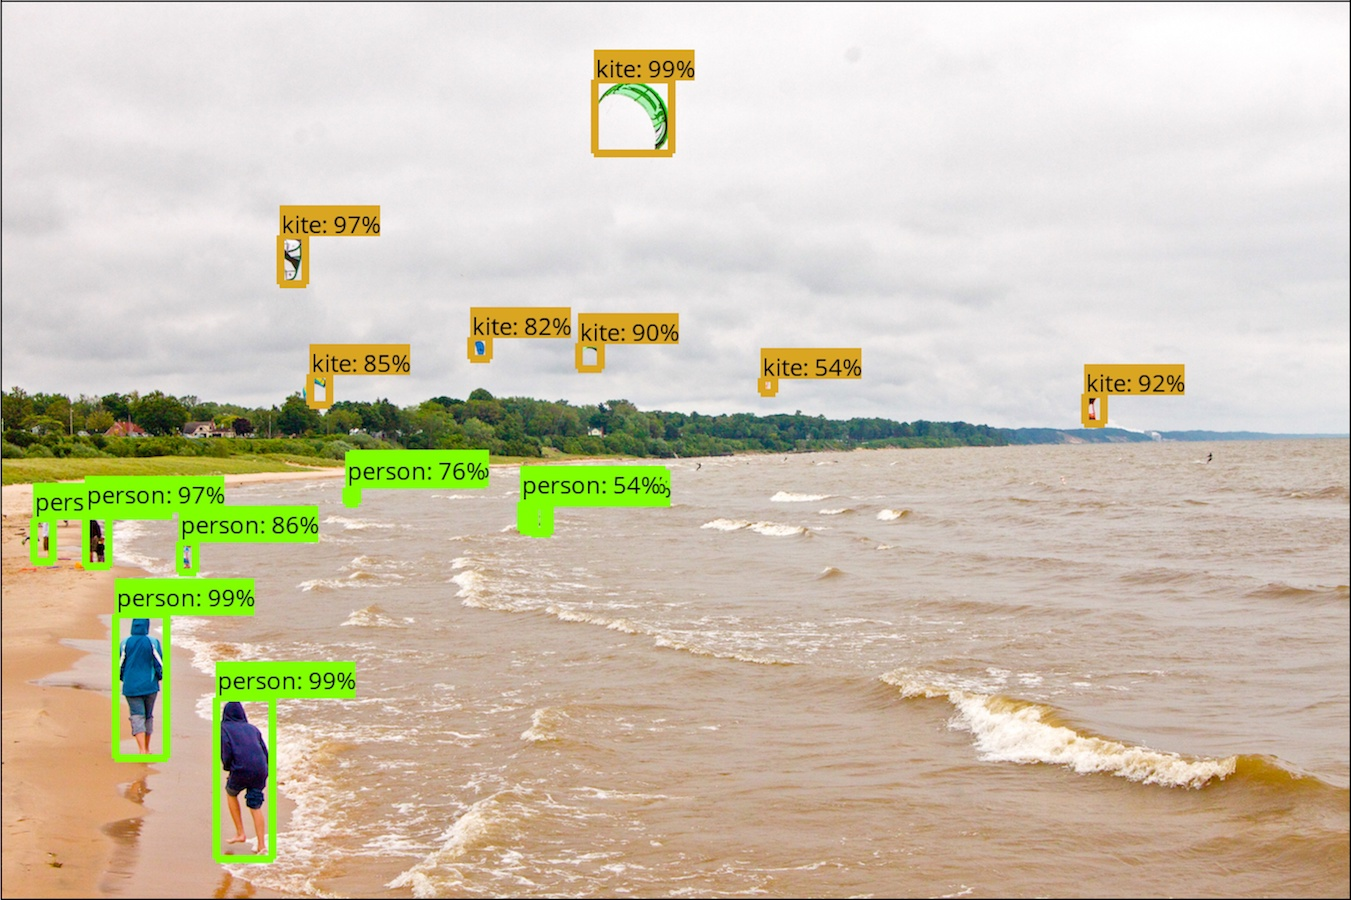
\includegraphics[width=0.8\columnwidth]{kites_detections_output}
  \caption{Real-world object detection using bounding boxes, from
    \cite{huang_speed/accuracy_2016}. Class labels and confidence scores
    accompany each box. Objects detected with $> 50\%$ confidence shown.}
  \label{fig:real-world}
\end{figure}

\begin{figure}
  \centering
  \begin{subfigure}[b]{0.45\columnwidth}
    \includegraphics[width=\columnwidth]{image_8841}
    \caption{}
    \label{fig:bare-gyros}
  \end{subfigure}
  \hfill
  \begin{subfigure}[b]{0.45\columnwidth}
    \centering
    \includegraphics[width=\columnwidth]{thumbnail_000_8841}
    \caption{}
    \label{fig:single-bare-gyro}
  \end{subfigure} \\
  \begin{subfigure}[b]{0.45\columnwidth}
    \includegraphics[width=\columnwidth]{box_output_8841}
    \caption{}
    \label{fig:bounding-boxes}
  \end{subfigure}
  \hfill
  \begin{subfigure}[b]{0.45\columnwidth}
    \includegraphics[width=\columnwidth]{shifted_box_output_8841}
    \caption{}
    \label{fig:bounding-boxes-shifted}
  \end{subfigure}
  \caption{In (\textbf{a}), the full gyroscopic model for topological
    metamaterials from \cite{nash_topological_2015}, where each individual gyro
    (\textbf{b}) is constrained to motion inside its circle. The center ``dot''
    is the object being tracked. In (\textbf{c}), the network from
    \cite{huang_speed/accuracy_2016} predicts bounding boxes for each gyro,
    using $16\times 16$ boxes centered on each gyro's ground truth position for
    training. Although each box bounds its dot, it does not center itself around
    the dot, preventing location inference. The network is resilient to a
    translational shift (\textbf{d}) of $60$ pixels. Note the lower confidence
    scores, with one gyro receiving $< 50\%$.}
  \label{fig:gyro-image}
\end{figure}

\section{Experiment}
\label{sec:experiment}

% Describing the dataset. Perhaps this requires its own section, with one
% paragraph describing the experiment and its goals, and another describing the
% properties of the video, which broken into training and testing sets
In particular, we apply DNNs to detect the $(x,y)$ image-space positions of $54$
gyroscopes in the experimental setup from \cite{nash_topological_2015}. A
single, $600\times 800$ video was used, with $7742$ frames extracted for the
training set, $1000$ for the test set. Fig. \ref{fig:bare-gyros} shows a typical
image from the full-image dataset, while Fig. \ref{fig:single-bare-gyro} shows a
cropped thumbnail of a single gyro, centered on its mean position. Each gyro is
marked with a painted white dot and restricted to move within a constant
circular area. This setup lends itself to traditional methods for object
localization, \emph{e.g.}  gradient ascent or blob detection, which provided
ground truth positions on which to train.

\subsection{First Approach}     % Need better section title
\label{sec:first-approach}
% Describe the work done with the box-detectors, significance of near-enough
% localization so that gradient ascent algorithms 

Given the availability of box-detection schemes in
\cite{huang_speed/accuracy_2016}, we first applied the same networks for gyro
detection. We defined a training set with a single non-background class,
``dot,'' and $16 \times 16$ boxes centered on the ground truth position of each
gyro. As can be seen in Fig. \ref{fig:bounding-boxes}, the Object Detection API
succeeds very well in bounding the gyros' positions, but it fails to predict
boxes \emph{centered} on those positions, making precise location inference
impossible. Nevertheless, it is evident that the API, although designed for
``real-world'' tasks where precision is not expected, learned a valuable task
for initial localization. Fig. \ref{fig:bounding-boxes-shifted} shows the
networks' relative resilience to translational perturbations of the data,
despite being trained on a non-perturbed dataset. From this point, more refined
methods may be employed, inside each box, to infer precise gyro position. These
include traditional methods, already mentioned, as well as the machine learning
approach discussed below.

% Need better section title. Is regression with CNN novel enough? Seems pretty
% basic.
\section{Regression using Convolutional Neural Networks on Small Thumbnails}
\label{sec:conv-regr}

\subsection{Design}
\label{sec:design}

% Discuss the various approaches, show figures, cite the achieved precisions,
% then discuss the fallibility of the dataset
In order to recover pixel-level precision of the gyroscope positions, we applied
a relatively shallow Convolutional Neural Network (CNN)
\cite{krizhevsky_imagenet_2012} to several datasets of cropped images, or
thumbnails, of a single gyro. The initial layer consisted of $32$ different
$5 \times 5$ kernels (over grayscale images), followed by four layers, each with
$64$ $3 \times 3$ kernels. These were followed by two $2048$ unit
fully-connected layers and a $2$ unit output layer. Unlike CNNs designed for
classification tasks, which generally employ pooling layers to reduce the
dimensionality of the image and to introduce translational invariance to the
network, we retained full image dimension until the fully connected
layer. Admittedly, this approach is computationally expensive for larger images,
requiring the ``first-shot'' approximation that networks such as those in
\cite{huang_speed/accuracy_2016} provide. For this reason, we worked with the
cropped datasets described below.

\subsection{Datasets}
\label{sec:datasets}

In each dataset, we created one thumbnail from each image in the original
video. Thus each training set consisted of $7742$ training and $1000$ test
examples.

The first dataset, called the \emph{centered} set, consisted of $12 \times 12$
thumbnails fixed on the mean ground-truth position of a single gyro in
each. Since the gyro's dot is about $12$ pixels in diameter, it nearly fills the
image in every example, making the detection of its center a simple task. In the
second dataset, we used the same thumbnails and imposed a random, uniformly
distributed offset to create the $12 \times 12$ \emph{perturbed} dataset. In
each example, then, the ground-truth position of the gyro was off-center by up
to $4$ pixels in either direction. Additionally, any pixels outside of the
original centered thumbnail were replaced with Gaussian noise, ensuring that the
perturbations added no information not available to the centered
dataset. Finally, we replicated this process for $30 \times 30$ thumbnails, both
centered and perturbed. In the $30\times 30$ perturbed set, the ground truth
gyro position was off-center by up to $12$ pixels in either coordinate.

\subsection{Results}
\label{sec:results}

\begin{figure}
  \centering
  \begin{subfigure}[b]{0.49\columnwidth}
    \includegraphics[width=\columnwidth]
    {thumbnail_000_12x12_centered_images/centered_test_4}
    \caption{}
    \label{fig:thumbnail_000_12x12_centered_images/centered_test_4}
  \end{subfigure}
  \hfill
  \begin{subfigure}[b]{0.49\columnwidth}
    \includegraphics[width=\columnwidth]
    {thumbnail_000_12x12_centered_images/rand_bg_normal_test_3}
    \caption{}
    \label{thumbnail_000_12x12_centered_images/rand_bg_normal_test_3}
  \end{subfigure}\\
  \begin{subfigure}[b]{0.49\columnwidth}
    \includegraphics[width=\columnwidth]
    {thumbnail_000_30x30_rand_bg_normal_images/rand_bg_normal_test_4}
    \caption{}
    \label{thumbnail_000_30x30_rand_bg_normal_images/rand_bg_normal_test_4}
  \end{subfigure}
  \hfill
  \begin{subfigure}[b]{0.49\columnwidth}
    \includegraphics[width=\columnwidth]
    {thumbnail_000_30x30_rand_bg_normal_images/centered_test_4}
    \caption{}
    \label{thumbnail_000_30x30_rand_bg_normal_images/centered_test_4}
  \end{subfigure}
  \caption{Isolated gyro images from the test set. Ground truth predictions are
    marked in green, inferred positions in red. The network trained on the
    $12\times 12$ \emph{centered} dataset (\textbf{a}) achieves sub-pixel
    accuracy relative to ground truths on the centered test set. The same
    network performs poorly (\textbf{b}) when tested on randomly offset
    thumbnails with random noise background. The $30\times 30$ dataset with
    random perturbations and background noise (\textbf{c}) produces a resilient
    network that performs well on centered data, after learning on the perturbed
    set (\textbf{d}).}
  \label{fig:thumbnails}
\end{figure}

\begin{figure}
  \centering
  \begin{subfigure}[b]{0.49\columnwidth}
    \includegraphics[width=\columnwidth]
    {thumbnail_000_12x12_rand_bg_normal_images/rand_bg_normal_test_3}
    \caption{}
    \label{thumbnail_000_12x12_rand_bg_normal_images/rand_bg_normal_test_3}
  \end{subfigure}
  \hfill
  \begin{subfigure}[b]{0.49\columnwidth}
    \includegraphics[width=\columnwidth]
    {thumbnail_000_12x12_rand_bg_normal_images/dot_001_rand_bg_normal_test_3}
    \caption{}
    \label{thumbnail_000_12x12_rand_bg_normal_images/dot_001_rand_bg_normal_test_3}
  \end{subfigure}
  \caption{Test images from the perturbed dataset (\textbf{a}) show network
    performance for the gyro on which it was trained. That same network was
    tested on a perturbed test set from \emph{a different gyro} (\textbf{b}).}
  \label{fig:different-dot}
\end{figure}

For both the $12 \times 12$ and the $30\times 30$ datasets, we trained separate
networks on the centered set and the perturbed set, then tested on both training
sets. Fig. \ref{fig:thumbnail_000_12x12_centered_images/centered_test_4} shows
the prediction of the network trained on the centered set. As can be seen, the
network trained on centered data performs well on similarly centered data, with
a mean error distance of $0.4$ pixels across the test set (see Table
\ref{tab:network-performance}). However, the network fails to learn from the
desired features of the image, namely the ability to recognize the gyro dot
itself; it is incapable of recognizing the object far from the center of the
image. The predictions on the perturbed test, as in
Fig. \ref{thumbnail_000_12x12_centered_images/rand_bg_normal_test_3} set have a
mean error of $3.6$ pixels, which is almost the maximum random offset in that
test set. We hypothesize that this failure to learn the desired information
results from a low variation in the training data; the ground truth positions
had a variance of less than one pixel in either direction. As a result, the
network learns to guess in a constrained region around the center of the image.

Fig. \ref{thumbnail_000_30x30_rand_bg_normal_images/rand_bg_normal_test_4}, on
the other hand, shows the results of training on the perturbed dataset, this
time for the $30 \times 30$ dataset. The network performs with near-pixel
precision on both the perturbed set, on which it was trained, and the centered
set in Fig. \ref{thumbnail_000_30x30_rand_bg_normal_images/centered_test_4},
which it has never seen before. (We say near-pixel, despite having sub-pixel
average error, due to outliers.) In fact, it achieves better precision on both
datasets than the networks trained and tested on $12 \times 12$ images (see
Table \ref{tab:network-performance}). This suggests that the same network,
rather than being inhibited by larger images, was able to learn more information
from them.

Note, in particular, the precision of the network trained on the $30\times 30$
perturbed set when tested on the centered set. In this case, the perturbations
actually decreased the variance of predictions---from $0.2$, when trained on
centered data, to $0.1$---despite having to generalize over a wider range of
ground truths.

Finally, we tested the network trained on the $12 \times 12$ perturbed set on a
\emph{different} gyro, as shown in Fig. \ref{fig:different-dot}. Crucially, the
network performs comparably on this new gyro, despite having never seen it
during training. This suggests that a single network, trained on a dataset
generated from one object, may be used to detect similar objects \emph{without
  additional training}. The superior precision of the network trained on
perturbed datasets suggests that the principles employed in generating this
dataset significantly affect its performance. In this report, we explore the
effects of translational perturbations, but we propose that other perturbations
are essential for consistent precision in a laboratory experiment.

\begin{table*}[t]
  \centering
  \begin{tabular}{| c | c | c | c | c |}
    \hline
    Images & Training Set & Test Set & Mean Error Distance & Standard Deviation \\
    \hline
    \multirow{5}{4em}{$12 \times 12$}
                   & centered & centered & 0.3 & 0.2 \\
                   & centered & perturbed & 3.6 & 1.4 \\
                   & perturbed & perturbed & 0.8 & 0.4 \\
                   & perturbed & centered & 0.5 & 0.2 \\
                   & perturbed & perturbed (new gyro) & 0.8 & 0.4 \\
    \hline
    \multirow{4}{4em}{$30 \times 30$}
                   & centered & centered & 0.4 & 0.2 \\
                   & centered & perturbed & 9.7 & 1.4 \\
                   & perturbed & perturbed & 0.6 & 0.3 \\
                   & perturbed & centered & 0.4 & 0.1 \\
                   % & perturbed (QG) & perturbed (QG) & 9.3 & 3.5 \\
    \hline
  \end{tabular}
  \caption{Performance for various networks on individual cropped datasets, as
    in Figures \ref{fig:thumbnails} and \ref{fig:different-dot}. Networks
    trained on the perturbed dataset achieved sub-pixel accuracy.}
  \label{tab:network-performance}
\end{table*}

\subsection{Ground Truth Precision}
\label{sec:ground-truth-prec}

As can be seen in Figures \ref{fig:thumbnails} and \ref{fig:different-dot}, the
ground truth positions of the gyroscopes (shown in green) are less than
ideal. Intuitively, this can impede network generalization because it forces the
network to learn special cases seen in the training set where the ``true''
position of the gyro is not its center. Interestingly, despite these
limitations, we observed that the networks trained on the perturbed data tended
to make errors more toward the apparent center of the blob, when tested on the
centered data. That is, the predicted position, although offset from the
provided ground-truth position of the gyro, was very often closer to the actual
center of the gyro than the ground truth. This has potential implications for
the training of networks with greater precision than the data they train
on. However, it remains an area of exploration.

\section{Artificial Dataset Generation}
\label{sec:artif-datas-gener}
% Talk about artificial dataset generation, somehow include the graphic that
% Kindlmann wants to see.

\begin{figure}
  \centering
  \includegraphics[width=0.8\columnwidth]{dependencies}
  \caption{A directed graph modeling dependencies in the experiment. We propose
    that the source nodes in such a graph determine which qualities should be
    perturbed in an artificial dataset.}
  \label{fig:dependencies}
\end{figure}

The usefulness of the machine learning approach in a laboratory setting is
largely dependent on the availability of ground truths for training. In our
data, from \cite{nash_topological_2015}, careful construction of the
experimental setup makes object positions available through the application of
traditional methods, but in order to apply machine learning techniques to new
experiments, well-representative ground truths must be available through less
effort than traditional methods require. Here, we explore the generation of an
artificial dataset from very few representative images, as they apply to the
gyroscope setup in \cite{nash_topological_2015}. In this case, a single gyro
could be precisely located in small, ``seed'' dataset, which would populate a
larger dataset of generated images emulating the experimental setup. To the
degree that objects being tracked are visually similar, one seed set could be
used to train many networks, each suited for a different experimental setup.

In Sec. \ref{sec:results}, we explored the effects of translational
perturbations on the dataset. This models one aspect of the experiment which we
certainly want a network to be sensitive to, namely the actual position of the
object in the image. However, the predicted position of an object depends on
many factors in the experiment. In order to create a resilient network, these
variables should be replicated in the artificial dataset. For example, changes
in lighting can affect the precision of traditional blob detection; an
artificial dataset, then, should include random perturbations to the image
brightness in order to produce a resilient network. Other variables include
bright reflections in the image (specular highlights), object rotation, and
camera orientation. To the extent that these can be separated, we propose that
an artificial dataset should include perturbations of each.

It is vital, then, that the variables in an experimental setup be well
understood. Fig. \ref{fig:dependencies} shows how different variables in the
experiment depend on each other. The desired variable, ``Predicted Object
Position,'' has multiple dependencies, which are ``sources'' in the graph. The
random translations in Sec. \ref{sec:datasets} amount to perturbations of
``Object Position in World'' in the $12 \times 12$ datasets, since that was
roughly the size of the object. In the larger $30\times 30$ datasets,
translations more resembled a perturbation of ``Camera Orientation,'' since the
features surrounding the object were moved as well. A more comprehensive dataset
would include both perturbations.

\section{Conclusions}
\label{sec:conclusions}

We explored the application of machine learning methods in the analysis of
laboratory images from \cite{nash_topological_2015}. We acknowledged the
difficulty involved in obtaining reliable ground truths for these methods and
proposed, as a potential solution, the generation of artificial datasets through
random perturbations of several variables. Despite imperfections in the ground
truth positions, we showed in Table \ref{tab:network-performance} that
relatively shallow CNNs with no pooling layers can be remarkably effective for
locating objects in small images. When combined with less precise bounding-box
networks, such as those from \cite{huang_speed/accuracy_2016}, these CNNs can
provide an end-to-end machine learning approach to position detection.

\subsection{Future Work}
\label{sec:future-work}

Many aspects of laboratory image analysis with neural networks remains
unexplored. We aim to more fully explore the possible perturbations of a seed
dataset in order to determine which are most vital for the training of an
effective network. Additionally, we acknowledge the problem of position
verification for an experiment where, because a machine learning technique was
applied with an artificial training set, no ground truth positions are
available. Here, we propose that the variance of pixel values may be obtained as
function of distance from predicted position. A good prediction set, then, would
have low variance close to the predicted position. This and similar methods may
be employed to verify positional data once acquired.

\begin{acknowledgment}
  We thank William Irvine for access to his laboratory and data, with special
  thanks to Noah Mitchell for continued support regarding the data. Finally, we
  thank Yali Amit for input and guidance.
\end{acknowledgment}

\bibliographystyle{asmems4}
\bibliography{report}

\end{document}
%%% Local Variables:
%%% mode: latex
%%% TeX-master: t
%%% reftex-default-bibliography: "report.bib"
%%% End:
